\documentclass[a4paper, 12pt]{article}

\usepackage{geometry}
\geometry{left=2cm, right=2cm, top=2cm, bottom=2cm}

\usepackage{cmap}
\usepackage{mathtext} 
\usepackage[T2A]{fontenc}
\usepackage[utf8]{inputenc}
\usepackage[english,russian]{babel}	

\usepackage{amsfonts,amssymb,amsthm,mathtools}
\usepackage{amsmath}
\usepackage{icomma} 

\usepackage{graphicx} 
\graphicspath{{picturies/}}
\usepackage{wrapfig}

\usepackage{array,tabularx,tabulary,booktabs}
\usepackage{longtable}
\usepackage{multirow}

\usepackage{caption}
\captionsetup{labelsep=period}

\renewcommand{\phi}{\varphi}
\newcommand{\eps}{\varepsilon}
\newcommand{\parag}[1]{\paragraph*{#1:}}

\newcounter{Points}
\setcounter{Points}{1}
\newcommand{\point}{\arabic{Points}. \addtocounter{Points}{1}}

\author{Радькин Кирилл, Б01-005}
\date{5.03.22}
\title{Лабораторная работа 4.4.1. Амплитудная дифракционная решётка.}

\begin{document}
\maketitle

\parag {Цель работы} Знакомство с работой и настройкой гониометра Г5, определение спектральных характеристик амплитудной решётки

\parag {В работе используются} гониометр, дифракционная решётка, ртутная лампа

\parag{Внешний вид гониометра}~

\begin{figure}[!h]
    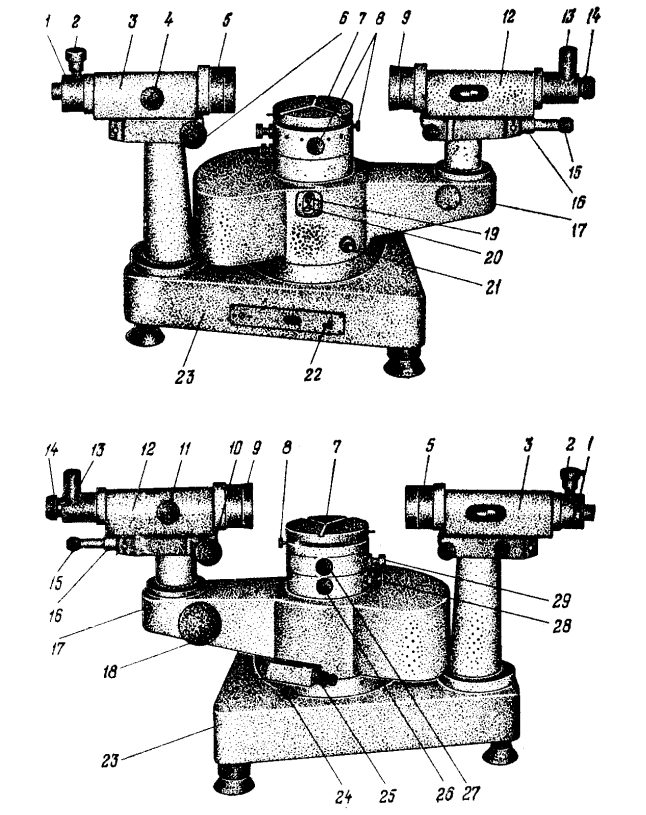
\includegraphics[scale = 0.4]{pic1.png}
    \centering
    \label{pic1}
\end{figure}

\parag {Теоретическое введение}

\begin{itemize}
    \item Интенсивность дифрагированного света максимальна для углов $\phi_m$, при которых волны, приходящие в точку наблюдения от всех щелей оказываются в фазе: 
    
    \begin{equation}
        \label{huinya1}
        d \sin \phi_m = m \lambda
    \end{equation}

    \item Угловая дисперсия $D(\lambda)$ характеризует угловое расстояние между близкими спектральными линиями:
    
    \begin{equation}
        \label{huinya2}
        D(\lambda) = \dfrac{d\phi}{d\lambda}
    \end{equation}

    В современных приборах спектроскопии регистрация изображения спектров проводится не глазом, а линейкой или матрицей чувствительных к свету элементов. Угловая дисперсия позволяет определить минимальное расстояние между ячейками приёмного устройства

    \item Рассмотрим изображения спектра для двух узких спектральных линий с длинами волн $\lambda$ и $\lambda + \delta \lambda$. Для минимального значения $\delta \lambda$, которое может быть определено по результатам измерений, вводят важнейшую
    характеристику спектрального прибора~---~разрешающую способность

    \begin{equation}
        \label{huinya3}
        R = \dfrac{\lambda}{\delta \lambda}
    \end{equation}

    \item Угловое расстояние между двумя линиями определяется дисперсией:
    
    \begin{equation}
        \Delta \phi \approx D \delta \lambda = \dfrac{m}{d \cos \phi_m} \delta \lambda
    \end{equation}

    Для сравнения между собой различных спектральных приборов Релей предложил приравнять полуширину $\delta \phi$ и расстояние между линиями $\Delta \phi$.Критерий Релея удобен для различных оценок. Согласно ему для дифракционных решёток разрешающая способность определяется порядком спектра и числом штрихов:

    \begin{equation}
        R = N m
    \end{equation}
\end{itemize}

\parag {Ход работы} ~

\begin{enumerate}
    \item Настроим установку
    \item Измерим угловые координаты спектральных линий ртути в $\pm 1$ порядке. Начальный угол $\phi_0 = 182^\circ 31' 50''$
    
    \begin{tabular}{|c|c|c|c|c|c|c|c|} \hline
        цвет & кр. 2 & желт. 1 & желт. 2 & зел. & гол. & син. & фиол. \\ \hline
        угол & $200^\circ 40’ 28’’$ & $199^\circ 21’ 1’’$ & $199^\circ 16’ 54’’$ & $198^\circ 22’ 28’’$ & $196^\circ 45’ 46’’$ & $195^\circ 6’ 43’’$ & $194^\circ 11’ 58’’$ \\ \hline
        цвет & фиол. & син. & гол. & зел. & желт. 2 & желт. 1 & кр. 2 \\ \hline
        угол & $171^\circ 51’ 42’’$ & $169^\circ 56’ 56’’$ & $168^\circ 18’ 33’’$ & $166^\circ 41’ 39’’$ & $165^\circ 45’ 4’’$ & $165^\circ 42’ 30’’$ & $164^\circ 22’ 30’’$ \\ \hline
    \end{tabular}

    \item Измерим угловую ширину линий желтого дуплета: \\
        левый край: $199^\circ 21’ 45’’$ \\
        правый край: $199^\circ 21’ 3’’$
\end{enumerate}

\parag {Обработка результатов} ~

\begin{enumerate}
    \item 

    \begin{figure}[!h]
        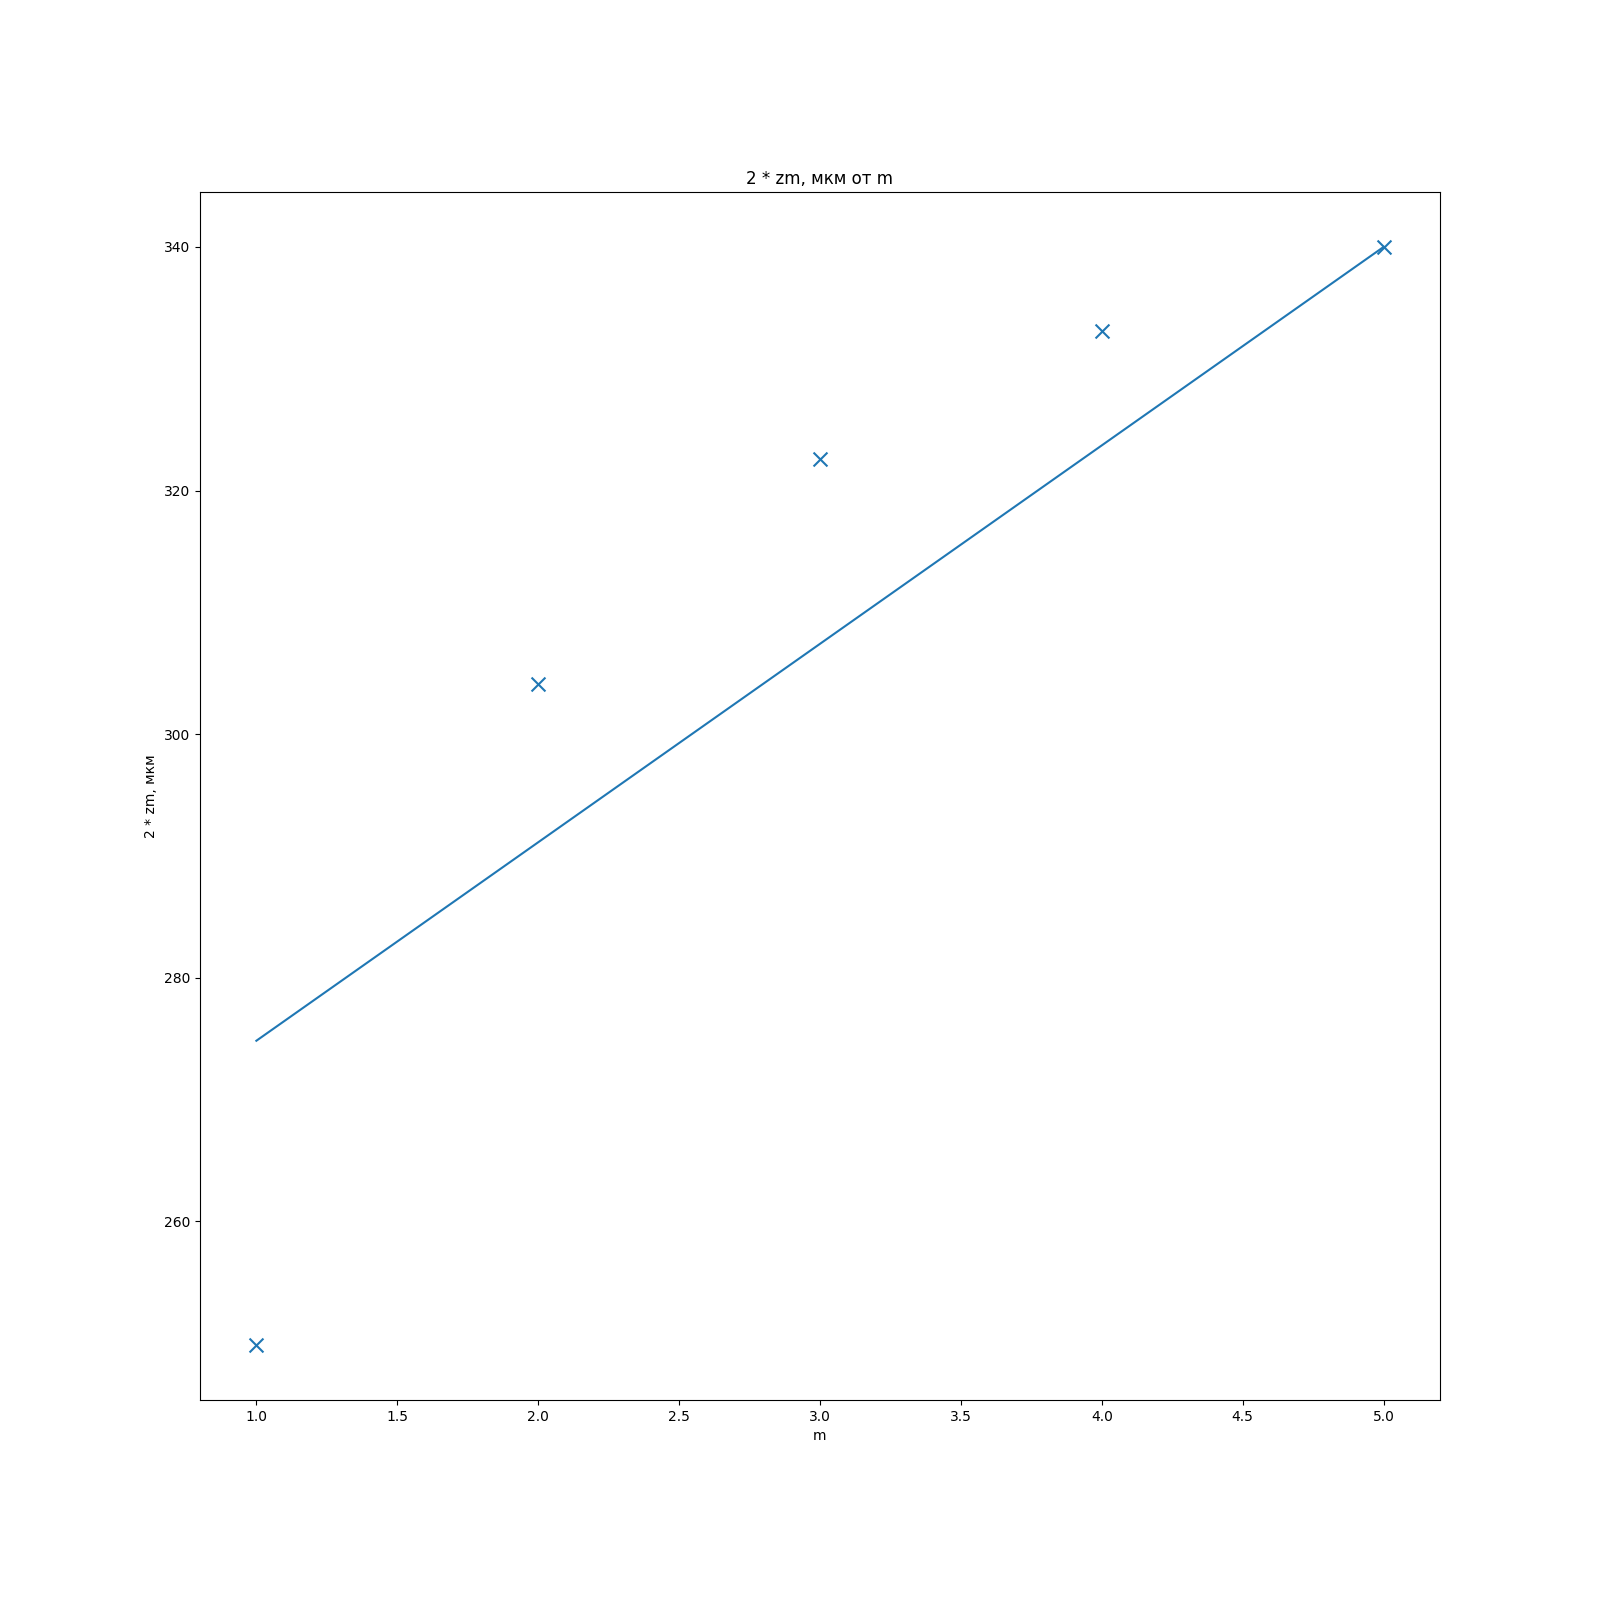
\includegraphics[scale = 0.4]{graph1.png}
        \centering
        \caption{$\sin \phi_m$ от $\lambda$}
        \label{graph1}
    \end{figure}

    Построим график зависимости $\sin \phi_m$ от длины волны (\ref{graph1}):

    Определим шаг решетки: $d_1 = 2003 \pm 2$ нм (для верхнего графика) и $d_2 = 2089 \pm 2$ нм (для нижнего графика), совпадает со значением, указанным на установке ($2$ мкм)

    \item Рассчитаем по линиям желтого дуплета угловую дисперсию в спектре 1 порядка: $D = 570.2 \pm 0.5 \dfrac{\text{рад}}{\text{мм}}$ 
    
    \item Оценим разрешимый спектральный интервал: $\delta \lambda = 0.357 \pm 0.003$ нм\\
    
    Оценим разрешающую способность для средней длины волны желтого дуплета ($580$ нм): $R = 1618.66 \pm 1.44$ \\

    Оценим число эффективно работающих штрихов: $\approx 1618$

    \item Рассчитаем порядок спектра, при котором фиолетоая линия наложится на желтую:
    
    $d \sin \phi = m \lambda_ж$, $d \sin \phi = (m + 1) \lambda_ф$ $\rightarrow$ $m \approx 2.34$
\end{enumerate}

\end{document}